% report.tex -- Discrete Event Simulation Analysis of a Web Application
\documentclass[10pt]{beamer}
\usetheme{Madrid}
\usecolortheme{beaver}

\usepackage{graphicx}
\usepackage{etoolbox}
\usepackage{booktabs}
\usepackage{amsmath,amssymb}
\usepackage{hyperref}
\usepackage{listings}
\usepackage{xcolor}

% Title info
\title[Discrete Event Simulation Analysis of a Web Application]{Discrete Event Simulation Analysis of a Web Application}
\subtitle{CS 681: Assignment 2}
\author[23b1035 \& 23b1067]{Sameer Arvind Patil(23b1035) \and Harsh Suthar(23b1067)}
\date{March 2026}

\begin{document}

% Title slide
\frame{\titlepage}

% Outline
\frame{
    \frametitle{Outline}
    \tableofcontents
}

\section{System Overview and Code overview}

\frame{
    \frametitle{System Overview}
    \begin{itemize}
        \item Multi-core web server simulator written in C++
        \item Models realistic web application performance characteristics
        \item Closed-loop user model: request $\to$ wait $\to$ think $\to$ repeat
        \item Thread-per-task model with configurable thread pool
        \item Supports multiple scheduling policies: Round-Robin (RR) and Shortest Job First (SJF)
        \item Discrete event simulation with warmup and transient removal
        \item Statistical analysis with confidence intervals
    \end{itemize}
}

\frame{
    \frametitle{Code Overview: Key Files}
    \begin{itemize}
        \item simulator.h -- main event loop, simulation lifecycle, RNG seed handling, warmup/steady-state management
        \item event.h -- event data structure, event types, priority ordering for the event queue
        \item core.h -- per-core scheduling, run-queue, dispatching to cores, scheduling policy implementation
        \item threadworker.h -- thread abstraction, context-switch handling, thread pool bookkeeping
        \item queueing\_system.h -- admission control, waiting queues, request enqueue/dequeue logic and drop policies
        \item request.h -- request metadata (ids, service requirement, timeout, retries), completion and timeout flags
        \item common.h, main.cpp -- shared types, configuration parsing, logging and metrics 
    \end{itemize}
    \textbf{For detailed documentation, refer the README.md in the simulator folder in the github repo}
}

% \frame{
%     \frametitle{Simulator and Event Responsibilities}
%     \begin{itemize}
%         \item Simulator: drives the discrete-event loop, schedules/dispatches events, collects metrics (response time, throughput, util)
%         \item Event: timestamped actions (arrival, start, end, timeout, preempt), stored in a min-priority event queue
%         \item Event handling: each event delegates to appropriate subsystem (queueing system, core, threadworker)
%     \end{itemize}
% }

% \frame{
%     \frametitle{Core, ThreadWorker and Queueing System}
%     \begin{itemize}
%         \item Core: holds per-core run queue, implements scheduling policy (RR, SJF), accounts busy/idle time
%         \item ThreadWorker: represents a runnable thread, executes requests for a time-slice, applies context-switch overhead and quantum logic
%         \item QueueingSystem: decides admission, maps requests to cores or global queue, handles drops when pool is full
%     \end{itemize}
% }

% \frame{
%     \frametitle{Request, Enums and Metrics}
%     \begin{itemize}
%         \item Request: encapsulates service-time sampling, timeout window, user id and lifecycle timestamps (arrival, start, complete)
%         \item Enums: EventType (ARRIVAL/START/COMPLETE/TIMEOUT/PREEMPT), SchedulingPolicy (RR, SJF), RequestState
%         \item Metrics: accumulated statistics (response time distributions, goodput/badput, timeouts, core utilizations, drop rates) updated on request completion or timeout
%     \end{itemize}
% }
    % \begin{itemize}
    %     \item \textbf{Simulation class} \\
    %     \begin{enumerate}
    %         \item Handles all the events, invocating the required methods from other objects to process the events
    %     \end{enumerate}

        
    %     % \item \textbf{Cores}: Users generate requests in closed loop
    %     % \item \textbf{Admission Control}: Requests admitted to waiting queue if thread available
    %     % \item \textbf{Thread Execution}: Threads execute requests with time slicing (quantum)
    %     % \item \textbf{Timeouts}: Long-running requests timeout after specified duration
    %     % \item \textbf{Completion}: Requests complete, thread returns to pool, user thinks
    %     % \item \textbf{Collection}: Metrics collected after warmup period
       
    % \end{itemize}

% \frame{
%     \frametitle{Key Components}
%     \begin{columns}[T]
%         \column{0.5\textwidth}
%         \textbf{Request Model:}
%         \begin{itemize}
%             \item Service time (configurable distribution)
%             \item Timeout (uniform range)
%             \item User ID and request ID
%             \item Retry tracking
%         \end{itemize}
        
%         \column{0.5\textwidth}
%         \textbf{Core and Threading:}
%         \begin{itemize}
%             \item Multiple cores (configurable)
%             \item Thread pool with max limit
%             \item Per-core run queue
%             \item Context-switching overhead
%         \end{itemize}
%     \end{columns}
% }

\frame{
    \frametitle{Key Performance Metrics}
    \begin{itemize}
        \item \textbf{Average Response Time}: Mean time from request arrival to completion (Timed out requests not considered)
        \item \textbf{Throughput}: Total requests completed per second (goodput + badput)
        \item \textbf{Goodput}: Requests completed before timeout per second
        \item \textbf{Badput}: Timed-out requests completed per second
        \item \textbf{Timeout Rate}: Number of requests exceeding timeout threshold
        \item \textbf{Core Utilization}: Fraction of time cores are busy
        \item \textbf{Request Drop Rate}: Requests rejected due to full queue
    \end{itemize}
}

% ========================================
% Section 2: Setup 1 - MVA vs Simulation vs Assignment 1
% ========================================
\section{Setup 1: Simulated vs MVA vs Assignment-1}

\frame{
    \frametitle{Setup 1: Objective}
    \textbf{Question}: How well does the simulation match the Mean Value Analysis (MVA) theoretical model and Assignment 1 measurements?

    \vspace{0.3cm}
    This setup validates the simulator by comparing against:
    \begin{itemize}
        \item MVA theoretical predictions
        \item Empirical measurements from Assignment 1
        \item Single simulator run with Assignment 1 parameters
    \end{itemize}
}

\frame{
    \frametitle{Setup 1: Parameters}
    \begin{table}
        \footnotesize
        \centering
        \begin{tabular}{ll}
            \toprule
            \textbf{Parameter} & \textbf{Value} \\
            \midrule
            Number of Users & 10 to 295 (step 20) \\
            Service Time Distribution & Constant 30 ms \\
            Number of Cores & 1 \\
            Max Threads & 345 \\
            Quantum (time slice) & 10 ms \\
            Context Switch Overhead & 0.0 ms \\
            Think Time (base) & 4000 ms \\
            Think Time (exponential mean) & 10 ms \\
            Timeout Range & 30000--30010 ms \\
            Simulation Time & 180 seconds (warmup: 20 sec) \\
            \bottomrule
        \end{tabular}
    \end{table}
}

% \frame{
%     \frametitle{Setup 1: Rationale}
%     \begin{itemize}
%         \item \textbf{Single Core}: Matches Assignment 1 empirical measurements
%         \item \textbf{Constant Service Time}: Simplifies validation; removes variability
%         \item \textbf{Large Thread Pool}: Ensures thread availability across user ranges
%         \item \textbf{High Timeout}: With small service times, timeouts rarely occur
%         \item \textbf{Think Time Model}: Think time has mode (4000 ms) + exponential component (10 ms)
%         \item \textbf{Long Simulation}: Ensures steady-state metrics are accurate
%     \end{itemize}
% }


\frame{
    \frametitle{Setup 1: Comparison Results}
    \begin{center}
        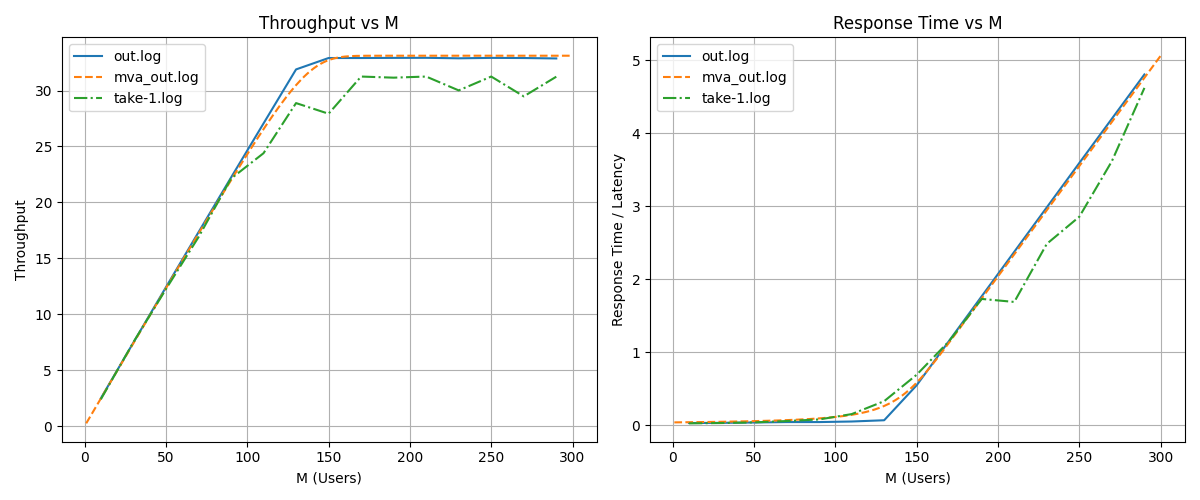
\includegraphics[width=0.9\textwidth]{plots/MVAvsSIMvsASS1.png}
    \end{center}
    \small
    The plot compares:
    \begin{itemize}
        \item \textbf{MVA}: Theoretical prediction line : mva\_out.log
        \item \textbf{Assignment 1}: Measured data from real system : take-1.log
        \item \textbf{Simulation}: Discrete event simulation results : out.log
    \end{itemize}
    }
    
    \frame{
    \frametitle{Analysis}
        \small
    
                \textbf{What the plot shows}
                \vspace{0.3em}
                \begin{itemize}
                    \item Throughput increases nearly linearly for small values of $M$.
                    \item After about 150 users, throughput starts to saturate, indicating system capacity limits.
                    \item Response time remains low initially, but rises sharply as the load increases.
                    \item The simulation output (\texttt{out.log}) is very close to the theoretical MVA prediction (\texttt{mva.out.log}).
                    \item The real measurement data (\texttt{take-1.log}) follows the same trend, but shows slightly more variation due to real-system effects.
                \end{itemize}
    
                \vspace{0.5em}
                \textbf{Conclusion}
    
                The three curves validate the model: the simulator and MVA match closely, and the measured system exhibits the expected performance trend.
        
    }
    
    % \frame{
    %     \frametitle{Setup 1: Analysis}
    %     \begin{itemize}
    %         \item Simulation closely matches MVA theoretical predictions
    %         \item Both show linear increase in response time with user load
    %         \item Simulation validates the core algorithm and event handling
    %         \item Small deviations from MVA due to:
    %         \begin{itemize}
    %             \item Discrete time-slicing effects
    %             \item Warmup transient removal
    %             \item Stochastic variations
    %         \end{itemize}
    %     \item Assignment 1 data may differ due to measurement methodology
    % \end{itemize}
% }

% ========================================
% Section 3: Setup 2 - Confidence Intervals
% ========================================
\section{Setup 2: Confidence Intervals on General Webserver}

\frame{
    \frametitle{Setup 2: Objective}
    \textbf{Questions}: 
    \begin{itemize}
        \item How do performance metrics scale with increasing user load?
        \item What are the confidence intervals for response time?
        \item Where does the system saturate?
    \end{itemize}
    
    \vspace{0.3cm}
    
    This setup performs 40 independent runs with varying user populations to compute statistically sound confidence intervals.
}

\frame{
    \frametitle{Setup 2: Parameters}
    \begin{table}
        \footnotesize
        \centering
        \begin{tabular}{ll}
            \toprule
            \textbf{Parameter} & \textbf{Value} \\
            \midrule
            Number of Users & 40 to 3000 (step 40) \\
            Service Time Distribution & Exponential, mean 60 ms \\
            Number of Cores & 4 \\
            Max Threads & 256 \\
            Quantum (time slice) & 10 ms \\
            Context Switch Overhead & 0.2 ms \\
            Think Time (base) & 3000 ms \\
            Think Time (exponential mean) & 200 ms \\
            Timeout Range & 20000--30000 ms \\
            Simulation Time & 180 seconds (warmup: 20 sec) \\
            Independent Runs & 40 \\
            Scheduling Policy & Round-Robin \\
            \bottomrule
        \end{tabular}
    \end{table}
}
\begin{frame}{Setup 2: Statistical Methodology}
\small

\begin{itemize}
    \item \textbf{Independent Replications:} 40 runs with different RNG seeds

    \item \textbf{Point Estimate:} Mean of the metric across all 40 runs for each user count

    \item \textbf{95\% Confidence Interval:}
    \[
    CI = \bar{X} \pm t_{0.025,39} \cdot \frac{S}{\sqrt{40}}
    \]
    where $S$ is the sample standard deviation across runs, and 
    $t_{0.025,39} \approx 2.02$ (Student’s t-distribution)

    \item \textbf{Warmup Removal:} First 20 seconds discarded (empirically chosen)

    \item \textbf{Transient Analysis:} Statistics collected only after warmup (steady-state period)
\end{itemize}

\end{frame}



\frame{
    \frametitle{Setup 2: Response Time Results}
    \begin{center}
        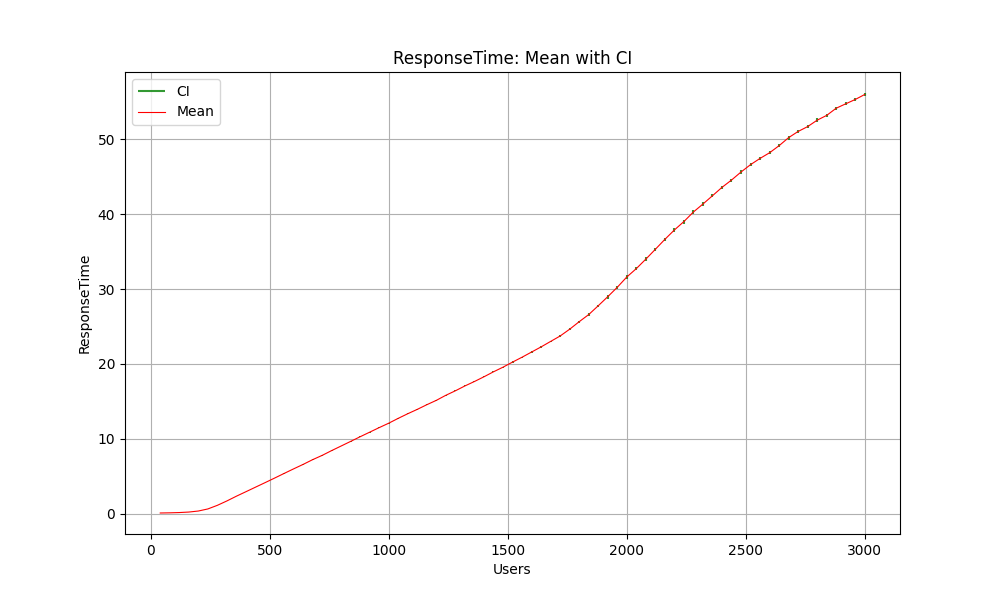
\includegraphics[width=0.9\textwidth]{confidence_interval/plots/ResponseTime.png}
    \end{center}
    \small
    \begin{itemize}
        \item Response time increases sub-linearly up to ~500 users
        \item Increase in response time and confidence interval at high loads
        \item Saturation point near 220 users
    \end{itemize}
}

\frame{
    \frametitle{Setup 2: Throughput Results}
    \begin{center}
        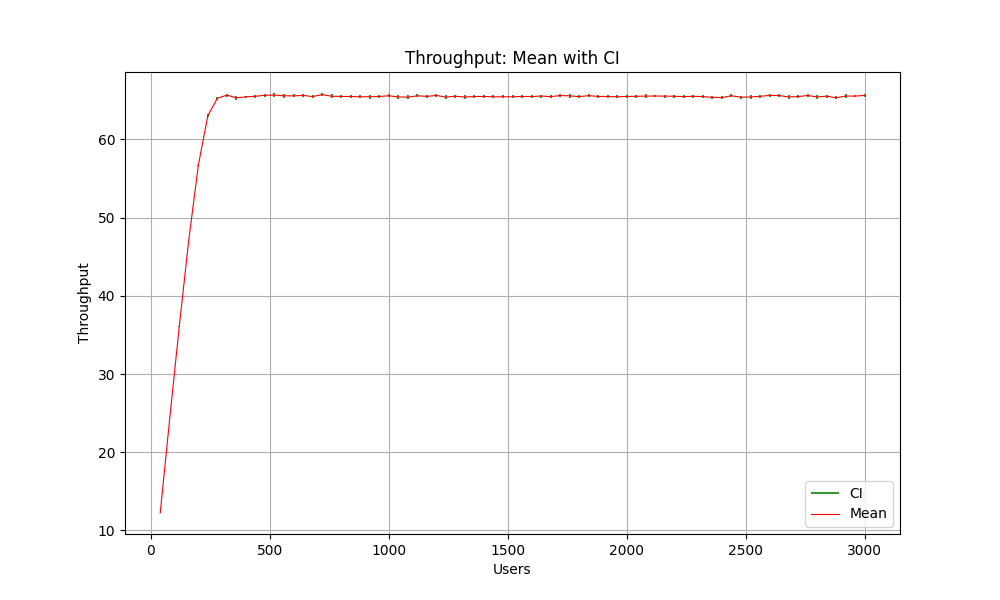
\includegraphics[width=0.9\textwidth]{confidence_interval/plots/Throughput.png}
    \end{center}
    \small
    \begin{itemize}
        \item Throughput increases with users up to saturation point
        \item Peak throughput $\approx$ 66 requests/sec at moderate load
        \item Plateaus after saturation due to server saturation
    \end{itemize}
}

\frame{
    \frametitle{Setup 2: Goodput vs Badput}
    \begin{center}
        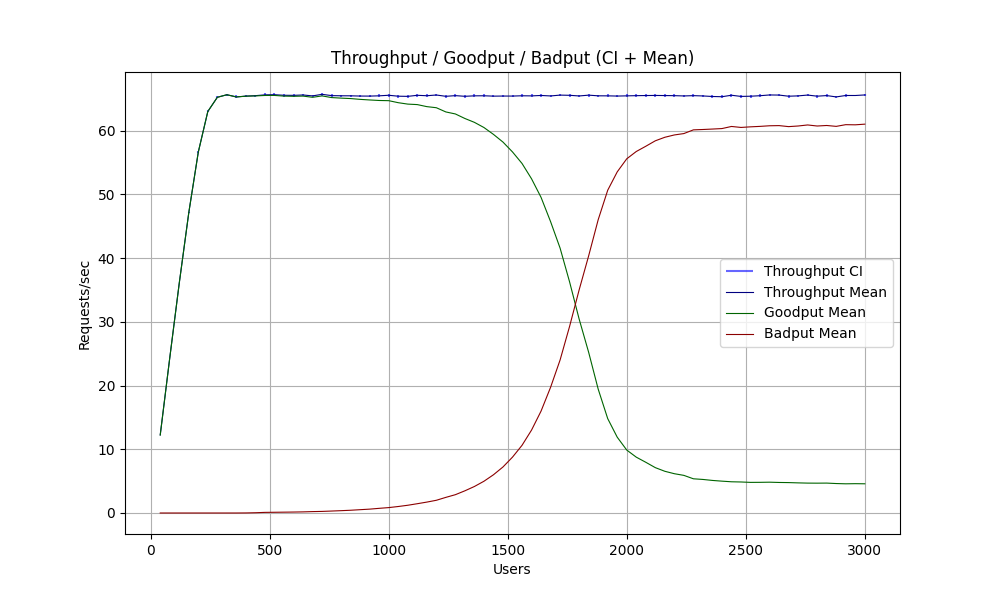
\includegraphics[width=0.9\textwidth]{confidence_interval/plots/throughput_goodput_badput.png}
    \end{center}
    \small
    \begin{itemize}
        \item Goodput:  left to be done
        \item Badput: Timed-out requests that still completed
        \item Badput grows significantly with load (requests queue too long)
    \end{itemize}
}

\frame{
    \frametitle{Setup 2: Utilization Results}
    \begin{center}
        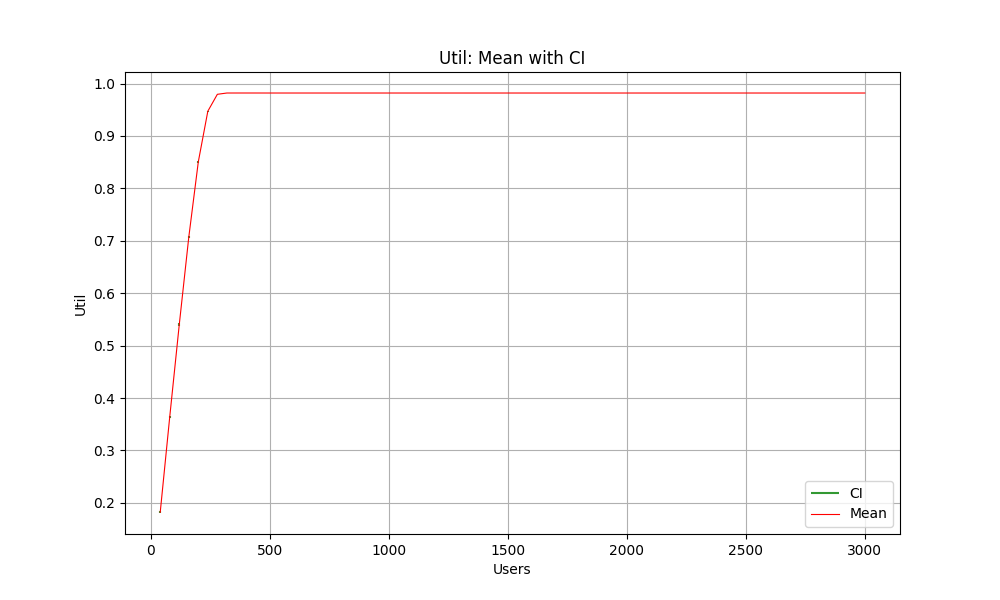
\includegraphics[width=0.9\textwidth]{confidence_interval/plots/Util.png}
    \end{center}
    \small
    \begin{itemize}
        \item Core utilization increases with user load untill saturation
        \item Reaches $\approx 95\%$ at saturation (Did not achieve 100\% utilization because of resources used in context-switches)
    \end{itemize}
}

\frame{
    \frametitle{Setup 2: Timeout Analysis}
    \begin{center}
        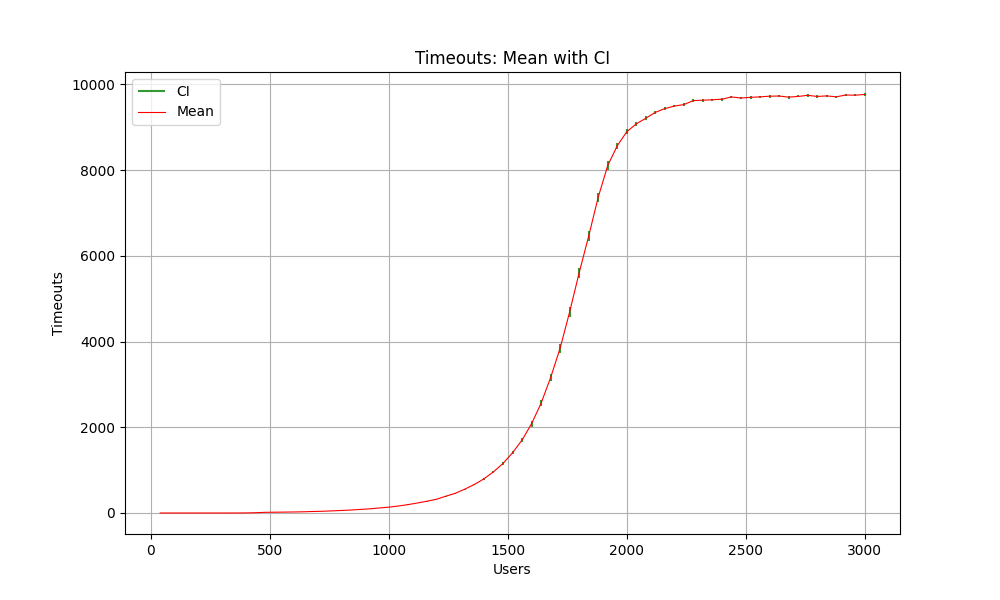
\includegraphics[width=0.9\textwidth]{confidence_interval/plots/Timeouts.png}
    \end{center}
    \small
    \begin{itemize}
        \item Few timeouts at low load  left to be done
        \item Exponential growth in timeouts above 1000 users
        \item System SLA violation indicates saturation
    \end{itemize}
}

\frame{
    \frametitle{Setup 2: Key Insights}
    \begin{itemize}
        \item \textbf{Saturation Point}: System becomes resource-constrained around 250 users
        \item \textbf{Queueing Effects}: Visible degradation in response time and goodput
        \item \textbf{Thread Pool Limit}: 256 threads insufficient for extreme loads
        \item \textbf{Variability}: Confidence intervals widen significantly at high loads
        \item \textbf{Confidence}: 95\% CI indicates statistical soundness lefttt
    \end{itemize}
}

% ========================================
% Section 4: Setup 3 - Scheduling Policy Comparison
% ========================================
\section{Setup 3: Scheduling Policy Comparison (RR vs SJF)}

\frame{
    \frametitle{Setup 3: Objective}
    \textbf{Questions}:
    \begin{itemize}
        \item How much does scheduling policy impact performance?
        \item Is SJF better than RR for web server workloads (in terms of response time)?
    \end{itemize}
    
    \vspace{0.3cm}
    
    This setup compares two scheduling policies:
    \begin{itemize}
        \item \textbf{Round-Robin (RR)}: Fair, simple scheduling
        \item \textbf{Shortest Job First (SJF)}: Prioritizes shorter jobs
    \end{itemize}
}

\frame{
    \frametitle{Setup 3: Parameters}
    \begin{table}
        \footnotesize
        \centering
        \begin{tabular}{lll}
            \toprule
            \textbf{Parameter} & \textbf{RR} & \textbf{SJF} \\
            \midrule
            Number of Users & 5--3000 (step 10) & 5--3000 (step 10) \\
            Service Time & Exp(60) ms & Exp(60) ms \\
            Number of Cores & 4 & 4 \\
            Max Threads & 256 & 256 \\
            Quantum &  10 ms & 100 ms \\
            Context Switch Overhead & 0.2 ms & 1.0 ms \\
            Think Time (base) & 3000 ms & 3000 ms \\
            Mean Think Time (exponential) & 200 ms & 200 ms \\
            Timeout Range & 20000--30000 ms & 20000--30000 ms \\
            \bottomrule
        \end{tabular}
    \end{table}
    Real think time is sum of base + exponential component.
}

\frame{
    \frametitle{Setup 3: Rationale}
    \begin{itemize}
        \item \textbf{Different Service Time}: Creates variability for SJF to optimize
        \item \textbf{Multiple Cores}: Real-world scenario with parallelism
        \item \textbf{Wide User Range}: Captures behavior from light to extreme load
    \end{itemize}
    We expect SJF to outperform RR in terms of response time. leftt
}

\frame{
    \frametitle{Setup 3: RR vs SJF Response Time}
    \begin{center}
        
\includegraphics[width=0.9\textwidth]{SJF_vs_RR/ResponseTime_vs_users.png}
    \end{center}
    \small
    \begin{itemize}
        \item SJF generally shows lower response time
    \end{itemize}
}

\frame{
    \frametitle{Setup 3: RR vs SJF Throughput}
    \begin{center}
        
\includegraphics[width=0.9\textwidth]{SJF_vs_RR/Throughput_vs_users.png}
    \end{center}
    \small
    \begin{itemize}
        \item Higher throughput for SJF
    \end{itemize}
}

\frame{
    \frametitle{Setup 3: Analysis}
    \begin{itemize}
        \item \textbf{SJF Advantage}: Better response time for short jobs
        \item \textbf{Saturation Behavior}: Both policies degrade similarly at extreme load
        \item \textbf{Recommendation}: 
            \begin{itemize}
                \item Use SJF for systems with highly variable service times
                \item RR is simpler and adequate for balanced workloads
                \item Consider hybrid approaches for critical services
            \end{itemize}
    \end{itemize}
}

% ========================================
% Section 5: Additional Analysis
% ========================================
\section{Additional Analysis and Future Work}

% \frame{
%     \frametitle{Potential Analysis Directions}
%     \begin{itemize}
%         \item \textbf{Timeout Parameter Sensitivity}: How do different timeout ranges affect goodput?
%         \item \textbf{Thread Pool Sizing}: Optimal thread pool size vs. memory cost
%         \item \textbf{Quantum Effects}: Impact of time slice size on overhead vs. fairness
%         \item \textbf{Service Time Distribution}: Compare constant, uniform, and exponential
%         \item \textbf{Think Time Impact}: Effects of think time distribution on load cycles
%         \item \textbf{Multiple Cores}: Scalability analysis with varying core counts
%     \end{itemize}
% }

% \frame{
%     \frametitle{Queue Dynamics Analysis}
%     \begin{itemize}
%         \item \textbf{Queue Length Distribution}: Measure average queue depth over time
%         \item \textbf{Wait Time Components}: Break down response time into:
%             \begin{itemize}
%                 \item Queueing delay (waiting for thread)
%                 \item Service delay (on core)
%                 \item Context-switching overhead
%             \end{itemize}
%         \item \textbf{Starvation Detection}: Identify which requests timeout most frequently
%         \item \textbf{Load Balancing}: Core utilization balance across all cores
%     \end{itemize}
% }

% \frame{
%     \frametitle{System Tuning Recommendations}
%     \begin{itemize}
%         \item \textbf{Thread Pool}: Size based on 95th-percentile concurrent requests
%         \item \textbf{Quantum Selection}: Tune for balance between fairness and overhead
%         \item \textbf{Timeout Strategy}: Set timeout based on 99th-percentile response time
%         \item \textbf{Request Admission}: Reject requests early if queue too deep
%         \item \textbf{Priority Queuing}: VIP users or critical requests get preference
%         \item \textbf{Load Shedding}: Graceful degradation at extreme load
%     \end{itemize}
% }

\frame{
    \frametitle{Conclusion}
    \begin{itemize}
        \item \textbf{Simulator Validation}: Discrete event simulation closely matches MVA theory and experimental data
        \item \textbf{Performance Characterization}: Comprehensive metrics with confidence intervals
        \item \textbf{Scheduling Impact}: SJF outperforms RR for variable workloads (in term of response time and throughput)
    \end{itemize}
}

\frame{
    \frametitle{Code Structure}
    \begin{columns}[T]
        \column{0.5\textwidth}
        \textbf{Core Components:}
        \begin{itemize}
            \item \texttt{simulator.h/cpp}: Main event loop lefttt
            \item \texttt{request.h}: Request tracking
            \item \texttt{core.h/cpp}: Per-core scheduling
            \item \texttt{threadworker.h}: Thread abstraction
        \end{itemize}
        
        \column{0.5\textwidth}
        \textbf{Analysis:}
        \begin{itemize}
            \item \texttt{plot.py}: Basic metrics plotting
            \item \texttt{confidence\_plotter.py}: CI calculations
            \item \texttt{mix\_plot.py}: Multi-file plotter
            \item Scripts: Runner shells for all setups
        \end{itemize}
    \end{columns}
}

\end{document}
